\documentclass[main.tex]{subfiles}
\begin{document}
	
	\chapter{Knowledge}
		\chapterauthor{\vspace{5mm}Jeremias Thun, Fabian Rosenstock, Paul Schnipper}
		
		\section{OWL}
		The main class "EnduringThing-Localized" contains the subclasses for every physical object in the ontology that is currently used. The main class itself remained from the predecessor of SUTURO 19/20. Another goal is to change this for the next milestone and delete this main class since it is superfluous.
The reference to the RoboCup was removed as well to create a more general ontology. This was realized by renaming the class "Robocupitems" to "Item". The physical objects are then divided into different classes, which are based on the use of the objects. For that the following classes were used:
		
		\begin{itemize}
		\item CleaningSupply
		\item Clothes
		\item Electronic
		\item Furniture
		\item Groceries
		\item PersonalHygiene
		\item Receptacle
		\item Tableware
		\item Tool
		\item Toy
		\item Unknown
		\item WritingMaterial
		\end{itemize}
		
		One of the goals was that the object that is to be carried next is dependent on the confidence of the object class, color, and shape. In order to realize this goal regions and data property were added to the ontology. Classes that represented these properties of an object were once a subclass of "EnduringThing-Localized" but have been converted into independent classes instead.  


		\section{gripping\_subscriber}
		It implements the "\_\_init\_\_" function that initializes the gripper and the "callback" function to check constantly whether the status of the gripper has changed. If the gripper opend the "release\_object\_from\_gripper" function it calls the beliefstate to release the object from the gripper, if there is one. If the gripper closed the "attach\_object\_to\_gripper" function, it attaches the closest object to the gripper, if it is within reach.

		\section{URDF}
		
		\subsection{Idea}
		One of this years main goals for the SUTURO group was to allow modules to be more general and enable other RoboCup tasks.\\
		Knowledge's only responsibility is to remember all objects and their respective attributes to determine the exact position the object has to be moved to.\\
		Previous to this milestone, objects could only ever be either on the table or in the shelf. This was a problem for the "Clean-Up" challenge, in which objects can be found anywhere in the room and have to be placed inside a basket. This is why it was decided to completely rework the surfaces.pl file. Sadly it used a feature of KnowRob called SRDL. The Semantic Robot Description Language uses ontologies to describe mechanical features of a robot. Sadly th group does not have access to the URDF to SRDL allowing to compile the new representation of the room created by planning.\\
		Because of these reasons it was decided to use the KnowRob component URDFProlog. It is capable of loading URDF files into the rdf-store. Problems occurred when the group tried to use rdf\_urdf.pl in conjunction to knowrob\_memory. With this package loaded all quantitative information is stored in the mem-store instead, thus the decision was made to create a fork from KnowRob. In it rdf\_urdf.pl itself uses knowrob\_memory and mem\_store\_retrieve replacing rdf\_has. This version of KnowRob  can be found on github: \hyperref[https://github.com/JeremiasThun/knowrob]{\mbox{JeremiasThun/knowrob}}.\\
		
		\subsection{Surfaces.pl}
		Using the URDF-data in the surfaces.pl got rewriten.
		\newpage
		\lstset{language=Prolog,numbers=left}
		
		To use surfaces.pl, init.pl loads the URDF representing the room into the knowledgebase first, by executing rdf\_urdf\_load\_file.
		It then finds all surfaces big enough to support an object and by calling assert\_surface\_types the surfaces are stored and grouped by type. At this point the ground is also created as a surface.\\
		
		
		\begin{lstlisting}
:- ros_package_path('knowledge', X),
	atom_concat(X, '/urdf/hsrb_lab.urdf', FileURL),
	kb_create(urdf:'Robot', Robot),
	rdf_urdf_load_file(Robot, FileURL).	
		
:- forall(supporting_surface(SurfaceLink),
	assert_surface_types(SurfaceLink)).
		\end{lstlisting}
		
		
		The type holds the information whether a surface is the source or the target. next\_object only looks for objects on surfaces set to source. What type is source can be set on-the-fly.\\
		
		Target surfaces can not be set at the moment, because the object\_goal\_pose does not yet support surfaces other then the 'old' shelf.\\
		
		The most effort was put in to create code that determines witch surface found objects are actually standing on. This works in two steps.\\
		First: For this the corners of the boxes representing surfaces are projected into a 2D plane. Using the X and Y position of the object and properties of triangles and rectangles the validity is checked.\\
		Second: If the objects is inside the 2D plane the Z coordinates are compared. When the position is above the surface within a certain threshold the object is asserted as being on this surface.\\
		When there is no surface found on which the object is standing on and the object is low enough in the world, the object is asserted to be on the ground.\\
		
		
		\subsection{The new URDF file}
		
		\begin{figure}[H]
		\centering
		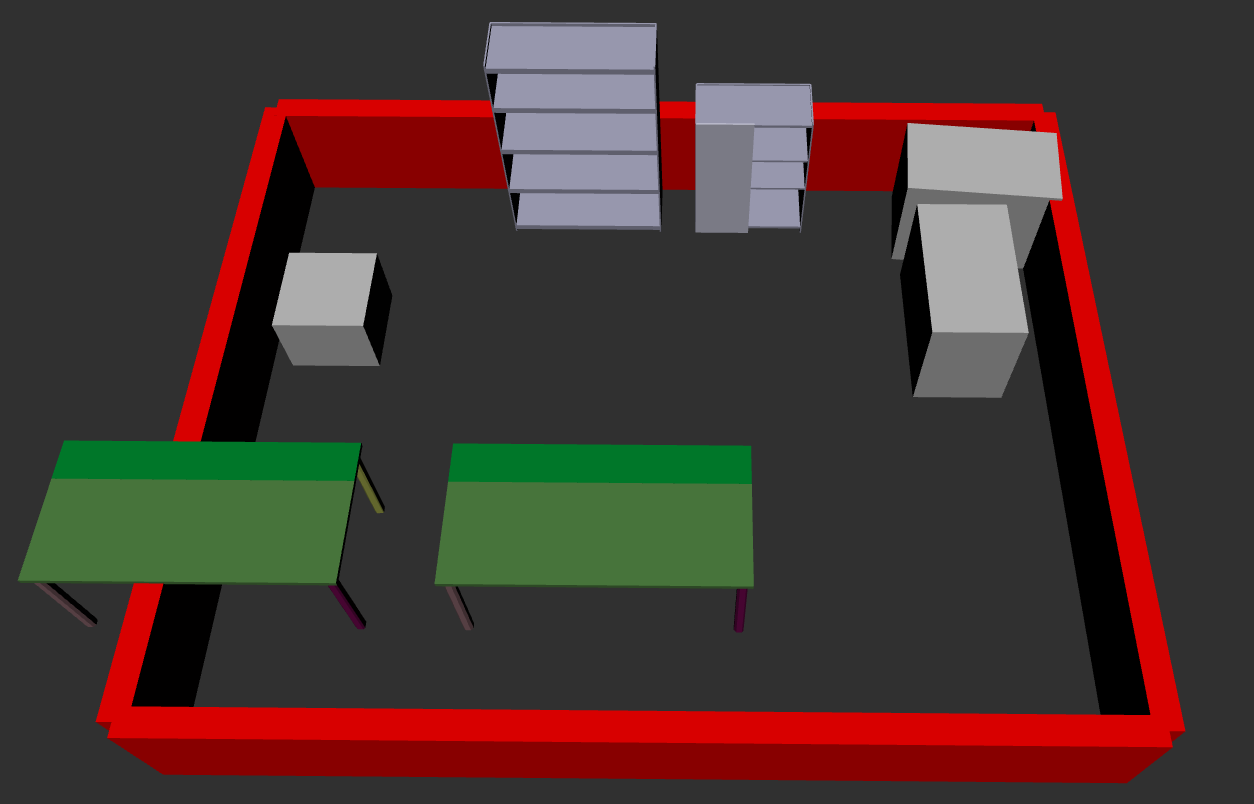
\includegraphics[width=0.7\linewidth]{pictures/knowledge_urdf.png}
		\caption{The current URDF.}
		\label{fig:knowledge_urdf}
		\end{figure}
		
		The new URDF file contains multiple tables and two shelf. The second, smaller shelf has  one door on it. In red are the walls. Surfaces.pl sees these as boxes, but their size is to small to be a supporting surface. They are only this high because in the RoboCup the arena will have similar low wall. A possible next step for knowledge might be the support for meshes. The two bigger tables in green are not URDF-boxes, so their size can not be determined by rdf\_urdf. This is why they are non existing for knowledge.\\
		To determine the position of the surface the current method is to add all parentjoints together. In the future using tf\_lookups will  simplify this.
		
		\subsection{Determining the goal position}
		
		As said previously one of the goals was that knowledge could freely based on information given by planning and the URDF decide where an object should be placed.\\
		Dew to time constrains the object\_goal\_surface and object\_goal\_pose functions where not reworked only adapted to use the new surfaces.
		
		

		\section{next\_object/1}
		The decision about which object should be the next to take is now part of Knowledge rather than Planning. The actual implementation does nothing more than returning the one object with the shortest distance to the robot at the moment. This calculation was moved to Knowledge to be able to start reasoning about other criteria when deciding what object to take. Some criteria that are being taken into consideration by this algorithm is:
		
\begin{itemize}
\item which known object classes are difficult to grip and should not be taken first?
\item which objects have no class at all, therefore are likely to be placed with the wrong cluster and should not be taken first?
\item which objects are in groups and therefore difficult to grip?
\item what is the confidence of the object class?
\item in case the object class is unknown and the object is placed based on it's color or size: What is the confidence of those attributes?
\end{itemize}

Since the robot's standing pose is supposed to depent on the next object rather than a specific spot that is hard coded, most objects should be reachable from a point in the map. 

		\section{Finding a place for the Objects}
		The decision about in which class to sort an object was refactored. In the old architecture the program would always look as far as the two previous branches in the hierachy. In the new architecture, the program asks for the class-distance in the OWL file and is able to define how much higher we need to go in the hierachy to get a match.\\
Another goal is to be able to have a full categorized picture of the shelf before the robot starts to put things inside. By approaching it like this, it is avoided that items that are placed in the shelf are sorted with the wrong groups, and the groups themselves ending up being mixed; partially sorted by class and partially sorted by attributes, which can vary extremely.
 

		\section{up-and-coming}
		One next step is to generify the different surfaces and their function. Depending on the challenge for the RoboCup, the same surface can be the source or the target. In order to be able to perform the clean up task the robot needs to go through every surface and look for objects to clean up. This functionality will be represented in the OWL-representation.\\
		Knowledge should also be able to tell planning all possible surfaces as points of interest, places it should look at to find misplaced objects.\\
		As a feature for Natural-Language-Generation grouping the shelf surfaces and finding descriptive names for them will be of use.\\
		Many of the classes, representing physical objects, belong to subclasses of "designed artifact" or other subclasses of the "physical object" class. The plan is to move these classes to the appropriate branch. In order to realize this, the prolog code needs to be adjusted since it uses the currently existing structure of the ontology.\\
		Another useful feature will be to have a way to forget all recognized objects, currently the knowledgebase has to be restarted for this, making testing more difficult. 


\end{document}
